\documentclass[a4paper,12pt]{article} % тип документа

% Поля страниц
\usepackage[left=2.5cm,right=2.5cm,
    top=2cm,bottom=2cm,bindingoffset=0cm]{geometry}
    
%Пакет дял таблиц   
\usepackage{multirow} 
    
%Отступ после заголовка    
\usepackage{indentfirst}


% Рисунки
\usepackage{floatrow,graphicx,calc}
\usepackage{wrapfig}

%%% Работа с картинками
\usepackage{graphicx}  % Для вставки рисунков
\graphicspath{{images/}{images2/}}  % папки с картинками
\setlength\fboxsep{3pt} % Отступ рамки \fbox{} от рисунка
\setlength\fboxrule{1pt} % Толщина линий рамки \fbox{}
\usepackage{wrapfig} % Обтекание рисунков и таблиц текстом

% Создаёем новый разделитель
\DeclareFloatSeparators{mysep}{\hspace{1cm}}

% Ссылки?
\usepackage{hyperref}
\usepackage[rgb]{xcolor}
\hypersetup{				% Гиперссылки
    colorlinks=true,       	% false: ссылки в рамках
	urlcolor=blue          % на URL
}


%  Русский язык
\usepackage[T2A]{fontenc}			% кодировка
\usepackage[utf8]{inputenc}			% кодировка исходного текста
\usepackage[english,russian]{babel}	% локализация и переносы




% Математика
\usepackage{amsmath,amsfonts,amssymb,amsthm,mathtools}

%%% Дополнительная работа с математикой
\usepackage{amsmath,amsfonts,amssymb,amsthm,mathtools} % AMS
\usepackage{icomma} % "Умная" запятая: $0,2$ --- число, $0, 2$ --- перечисление


% Что-то 
\usepackage{wasysym}


\begin{document}
\begin{center}
	\footnotesize{ФЕДЕРАЛЬНОЕ ГОСУДАРСТВЕННОЕ АВТОНОМНОЕ ОБРАЗОВАТЕЛЬНОЕ 			УЧРЕЖДЕНИЕ ВЫСШЕГО ОБРАЗОВАНИЯ}\\
	\footnotesize{МОСКОВСКИЙ ФИЗИКО-ТЕХНИЧЕСКИЙ ИНСТИТУТ\\(НАЦИОНАЛЬНЫЙ 			ИССЛЕДОВАТЕЛЬСКИЙ УНИВЕРСИТЕТ)}\\
	\footnotesize{ФАКУЛЬТЕТ ОБЩЕЙ И ПРИКЛАДНОЙ ФИЗИКИ\\}
	\hfill \break
	\hfill \break
	\hfill \break
	\hfill \break
\end{center}


\begin{figure*}[h]
    \centering
    \includegraphics*[width=10cm,height=7cm,keepaspectratio]{mipt_eng_text_png.png}
    \label{fig:my_label}
\end{figure*}


\begin{center}   
    \hfill \break
	\hfill \break
	\hfill \break
	\large{Лабораторная работа № 4.4.1\\ \hfill \break\Large{Амплитудная диффракционная решетка (гониометр)}}\\
	\hfill \break
	\hfill \break
	\hfill \break
	\hfill \break
	\begin{flushright}
		Баранов Даниил\\
		Группа Б02-103
	\end{flushright}
	\hfill \break
	\hfill \break
	\hfill \break
\end{center}
\hfill \break
\hfill \break
\hfill \break
\hfill \break
\begin{center}
	Долгопрудный, 2023 г.
\end{center}
\thispagestyle{empty}

\newpage

\textbf{Цель работы:} Знакомство с работой и настройкой гониометра Г5, определение спектральных характеристик амплитудной решётки.

\textbf{В работе используются:} гониометр, дифракционная решётка, ртутная лампа.

\floatsetup[table]{capposition=top}

\section{Теоретическая справка}

Основное соотношение приближенной теории дифракционной решётки:

	\begin{equation}
	d\sin \varphi_m = m\lambda.
 \label{main}
	\end{equation}
 
Угловая дисперсия $D$ характеризует угловое расстояние между близкими спектральными линиями:
	\begin{equation}
	D = \frac{d\varphi}{d\lambda} = \frac{m}{d \cos \varphi}=\frac{m}{\sqrt{d^{2}-m^{2} \lambda^{2}}}.
	\end{equation}

Рассмотрим изображения спектра для двух узких спектральных линий с длинами волн $\lambda$ и $\lambda+\delta\lambda$. Для минимального значения $\lambda+\delta\lambda$, которое может быть определено по результатам измерений, вводят важнейшую характеристику спектрального прибора — разрешающую способность:

\begin{equation}
    R=\frac{\lambda}{\delta\lambda}.
\end{equation}


\section{Экспериментальная установка}

\subsection{Устройство гониометра}

Гониометр служит для точного измерения углов и находит широкое применение в оптических лабораториях. С помощью гониометра можно определять показатели преломления и преломляющие углы призм и кристаллов, исследовать параметры дифракционных решёток, измерять длины волн спектральных линий и т. Д.

Оптическая схема гониометра представлена на рис. 1а. Свет от источника $S$ проходит через коллиматор (устройство, дающее параллельный пучок, состоящее из щели 1 и объектива 5 ) и преобразуется призмой или решёткой в набор параллельных пучков, каждый из которых соответствует определённой длине волны. Параллельные пучки со-

\begin{figure}[H]
    \centering
    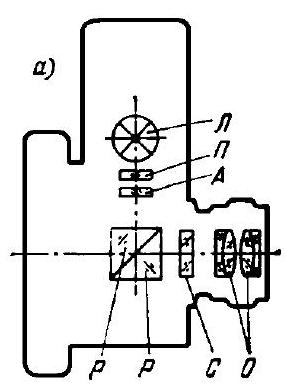
\includegraphics[scale=0.4]{2023_04_02_a48ae02e429ba186bcd7g-1(1)}

    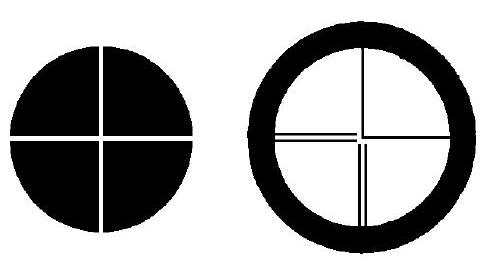
\includegraphics[scale=0.4]{2023_04_02_a48ae02e429ba186bcd7g-1}\\
    Рис. 2: Автоколлимационное устройство}
    \label{fig:my_label}
\end{figure}


бираются в фокальной плоскости объектива 9 зрительной трубы и рассматриваются глазом через окуляр 14. При освещении щели ртутной лампой, дающей дискретный спектр, в фокальной плоскости видны отдельные линии - цветные изображения входной щели (см. рис. 4 и таблицу 1).

Внешний вид гониометра представлен на рис. 16 и 1в. Коллиматор 3, столик 7 и алидада 17 со зрительной трубой 12 крепятся на массивном основании 23. На столике 7 размещаются исследуемые объекты. Коллиматор закреплён неподвижно, а столик и алидада с трубой могут вращаться вокруг вертикальной оси.

Ширину коллиматорной щели можно менять от 0 до 2-х мм при помощи микрометрического винта 2 , высоту - от 0 до 2-х см - при помощи диафрагмы с треугольным вырезом («ласточкин хвост»), надетой на щель. Винт 4 служит для перемещения объектива 5 - настройки коллиматора на параллельный пучок.

Зрительная труба 12 состоит из объектива 9 и окуляра 14 с автоколлимационным устройством 13. Объективы коллиматора и зрительной трубы одинаковы. Фокусировка трубы производится винтом 11. Наклон коллиматора и зрительной трубы к горизонтальной оси изменяется винтами 6 и 10 соответственно.

Схема окуляра О зрительной трубы с автоколлимационным устройством приведена на рис. 2а. Свет от лампы Л проходит через защитную стеклянную пластинку П и попадает на автоколлимационную сетку А, содержащую две взаимно перпендикулярные щели. Свет, прошедший через сетку А (светящийся крест - рис. 2б), попадает на две прямоугольные призмы $P$ и отражается от гипотенузной грани, на которую нанесён полупрозрачный слой с коэффициентом отражения $50 \%$.

Для юстировки гониометра на столик ставится предмет с плоской отражающей поверхностью. После отражения от неё 

A)
\begin{center}
    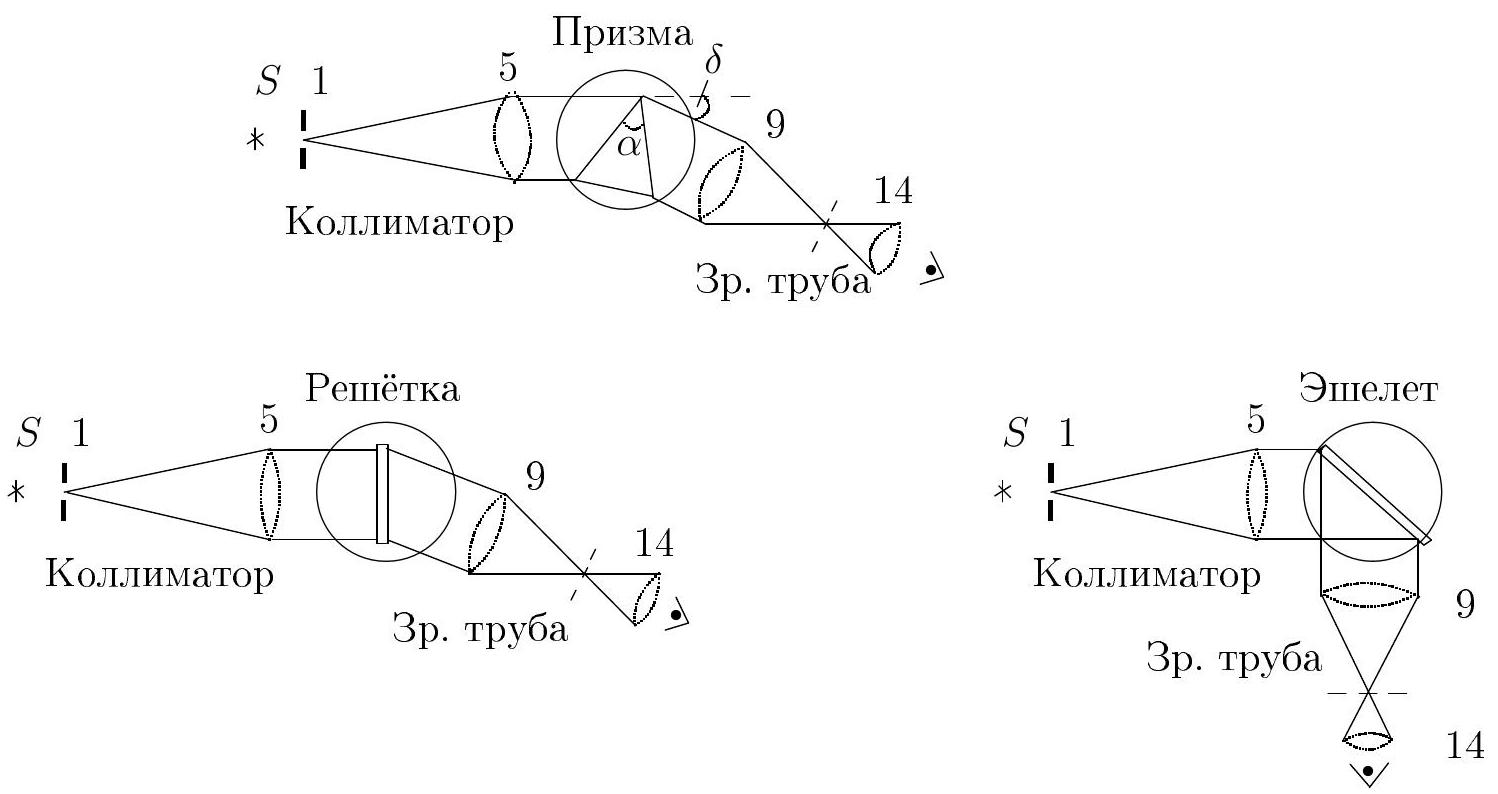
\includegraphics[scale=0.2]{2023_04_02_a48ae02e429ba186bcd7g-2}
\end{center}


Б)

\begin{center}
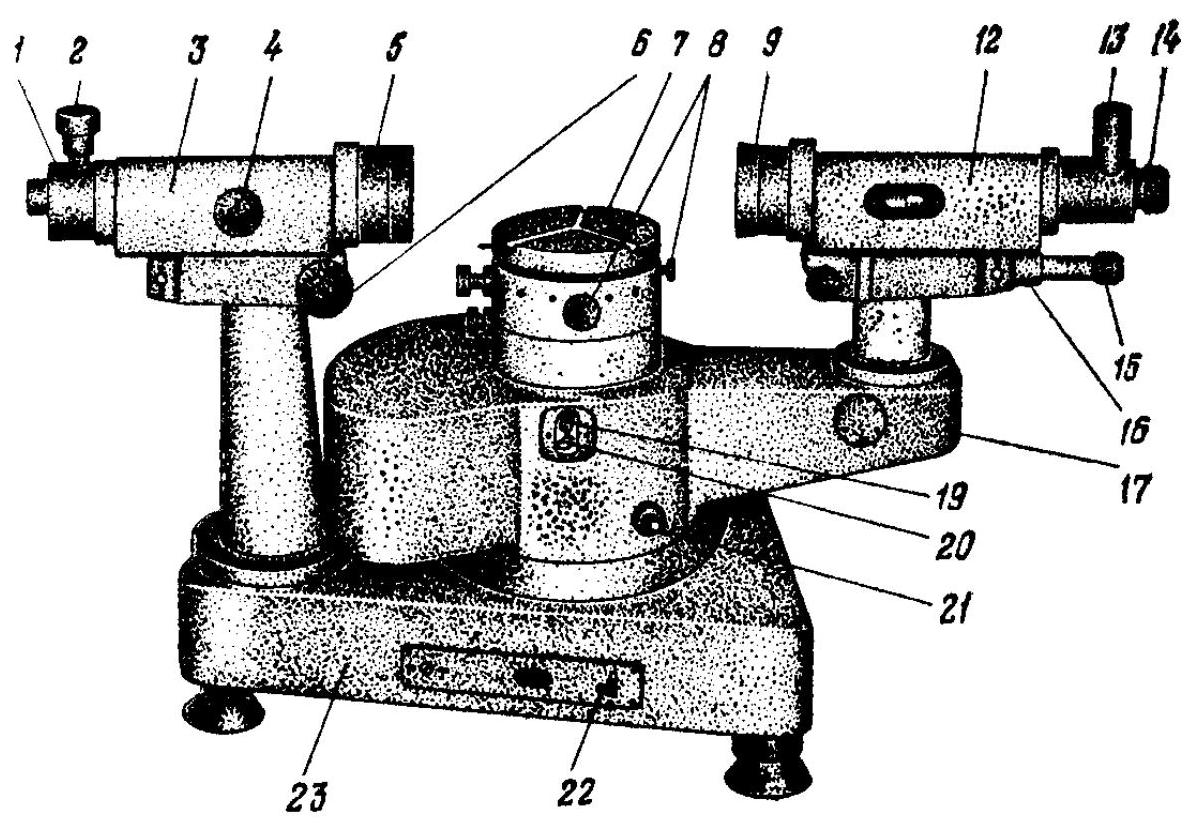
\includegraphics[scale=0.2]{2023_04_02_a48ae02e429ba186bcd7g-2(2)}
\end{center}

B)

\begin{center}
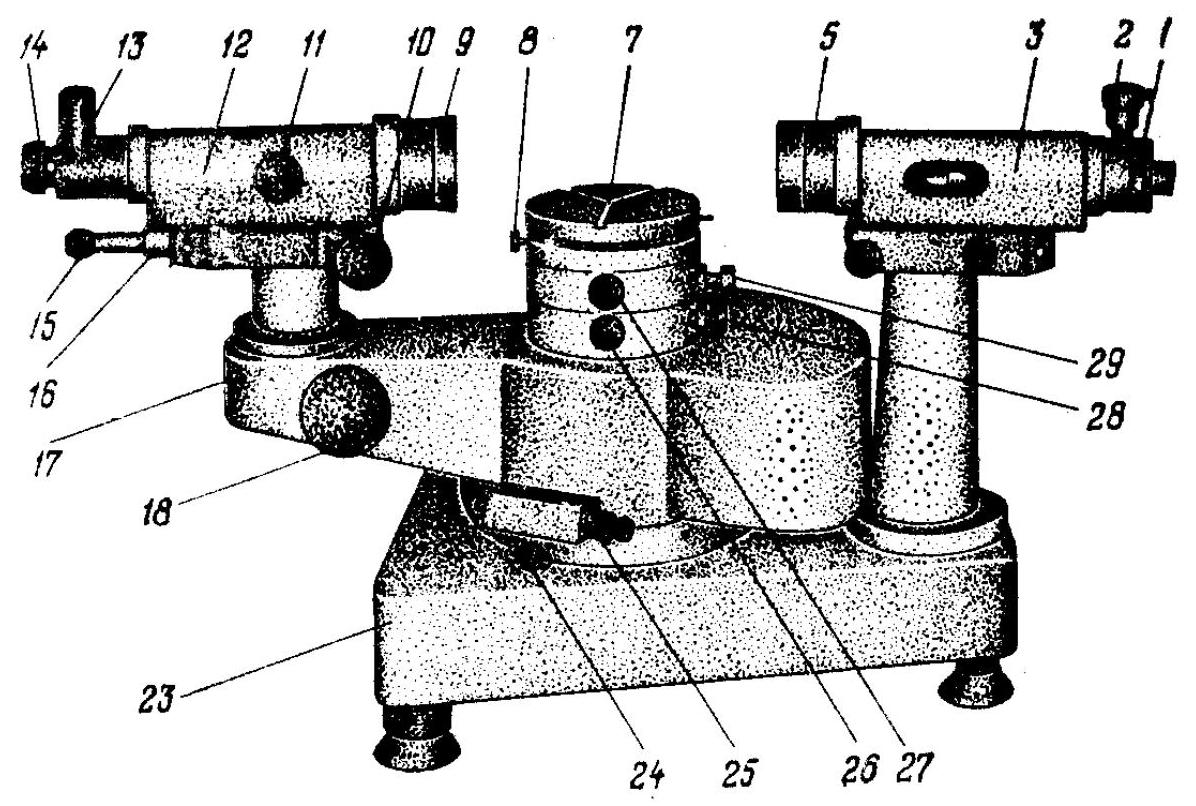
\includegraphics[scale=0.2]{2023_04_02_a48ae02e429ba186bcd7g-2(1)}

Рис. 1. Оптическая схема и внешний вид гониометра

\end{center}

 параллельный пучок лучей возвращается назад в зрительную трубу и собирается в фокальной плоскости объектива. В этом случае светящийся автоколлимационный крест можно увидеть через окуляр зрительной трубы. Кроме того, в окуляре имеется ещё одна сетка C, на которой изображён чёрный отсчётный крест (рис. 2в). Совмещённые изображения обоих крестов рассматриваются через окулярные линзы О. Резкость видимого изображения отсчётного креста регулируется вращением оправы окуляра трубы.

Обе сетки окуляра, А и C (рис. 2а), расположены на строго одинаковых расстояниях от гипотенузных граней призмы $P$, поэтому их одновременное наблюдение в окуляре возможно только при совпадении фокальных плоскостей объектива и окуляра (труба настроена на бесконечность).

Важнейшим узлом гониометра является устройство, служащее для отсчёта угла поворота зрительной трубы вокруг вертикальной оси, проходящей через центр столика. На этой оси крепится прозрачное кольцо (лимб), расположенное в корпусе прибора. На поверхности лимба нанесена шкала с делениями. Лимб разделён на $3 \times 360=1080$ делений. Цена деления $20^{\prime}$, оцифровка делений произведена через $1^{\circ}$. Шкалу лимба можно наблюдать через окуляр отсчётного устройства 16 при включённой подсветке (тумблер 22). Резкость изображения шкалы регулируется вращением оправы окуляра 15.

Оптическая система отсчётного устройства собрана так, что через окуляр можно наблюдать изображения штрихов двух диаметрально противоположных участков лимба, причём одно изображение прямое, а другое обратное (рис. 3). Кроме того, оптическая система позволяет перемещать эти изображения друг относительно друга, оставляя в покое как лимб, так и алидаду со зрительной трубой. Это перемещение штрихов измеряется при помощи оптического микрометра. Шкала микрометра рассчитана таким образом, что при перемещении её на 600 делений верхнее изображение штрихов лимба смещается относительно нижнего на 10'. Следовательно, цена деления шкалы микрометра $1^{\prime \prime}$.

Поле зрения отсчётного микроскопа приведено на рис. 3. В левом окне наблюдаются изображения диаметрально противоположных участков лимба и вертикальный штрих для отсчёта градусов, в правом - деления шкалы оптического микрометра и горизонтальная риска $R$ для отсчёта минут и секунд.

Для удобства экспериментатора в гониометре предусмотрено несколько вариантов относительного вращения столика, алидады со зрительной трубой и лимба.
Отсчётное устройство гониометра обеспечивает точность измерения угла не хуже $5^{\prime \prime}$.

\subsection{Ртутная лампа}

Характеристики спектра ртутной лампы ДРШ привдена в таблице

\begin{center}
\begin{tabular}{|c|c|c|c|c|c|c|c|c|}
\hline
№ & $\mathrm{K}_{1}$ & $\mathrm{~K}_{2}$ & 1 & 2 & 3 & 4 & 5 & 6 \\
\hline
$\lambda$ нм. & 690,7 & 623,4 & 579,1 & 577,0 & 546,1 & 491,6 & 435,8 & 404,7 \\
\hline
Цвет & красн. & красн. & желт. & желт. & зелен. & голуб. & синий & фиолет. \\
\hline
Яркость & 4 & 4 & 10 & 8 & 10 & 4 & 4 & 3 \\
\hline
\end{tabular}
\end{center}

\section{Ход работы}

Сначала были измерены углы для максимумов линий спектра ртутной лампы порядков $\pm 1$. Полученные данные приведены в таблице \ref{angles}.

\begin{table}[H]
    \centering
    \begin{tabular}{|p{2cm}|p{4cm}|p{4cm}|}
    \hline  \centering{№ линии} & $\varphi_{+1}$ &  $\varphi_{-1}$ \\ \hline
$6$   & $11^{\circ} 41^{\prime} 57^{\prime \prime}$  & $11^{\circ} 38^{\prime} 29^{\prime \prime}$  \\ \hline
$5$   & $12^{\circ} 36^{\prime} 34^{\prime \prime}$  & $12^{\circ} 33^{\prime} 37^{\prime \prime}$  \\ \hline
$4$   & $14^{\circ} 15^{\prime} 39^{\prime \prime}$  & $14^{\circ} 11^{\prime} 58^{\prime \prime}$  \\ \hline
$3$   & $15^{\circ} 52^{\prime} 33^{\prime \prime}$  & $15^{\circ} 48^{\prime} 17^{\prime \prime}$  \\ \hline
$2$   & $16^{\circ} 48^{\prime}  4^{\prime \prime}$  & $16^{\circ} 43^{\prime} 18^{\prime \prime}$  \\ \hline
$1$   & $16^{\circ} 51^{\prime} 56^{\prime \prime}$  & $16^{\circ} 47^{\prime} 1^{\prime \prime}$  \\ \hline
$K_2$ & $17^{\circ} 52^{\prime}  8^{\prime \prime}$  & $17^{\circ} 47^{\prime} 11^{\prime \prime}$  \\ \hline
$K_1$ & $18^{\circ} 12^{\prime} 43^{\prime \prime}$  & $18^{\circ}  6^{\prime } 48^{\prime \prime}$  \\ \hline

        
    
    \end{tabular}
    \caption{Углы линий спектра ртути}
    \label{angles}
\end{table}

Далее, для оценки угловой дисперсии решётки были измерены угловые координаты линий жёлтого дублета для всех видимых порядков спектра, положительных и отрицательных. Данные можно найти в таблице \ref{yell}.

\begin{table}[H]
    \centering
    \begin{tabular}{|c|p{4cm}|p{4cm}|}
    \hline $m$ & $\varphi_{2}$ & $\varphi_{1}$ \\ \hline
$1$   & $16^{\circ} 48^{\prime}  4^{\prime \prime}$  & $16^{\circ} 51^{\prime} 56^{\prime \prime}$  \\ \hline
$-1$  & $16^{\circ} 43^{\prime} 18^{\prime \prime}$  & $16^{\circ} 47^{\prime} 1^{\prime \prime}$  \\ \hline
$2$   & $35^{\circ} 24^{\prime} 15^{\prime \prime}$  & $35^{\circ} 33^{\prime} 12^{\prime \prime}$  \\ \hline
$-2$  & $35^{\circ}  3^{\prime} 45^{\prime \prime}$  & $35^{\circ} 12^{\prime} 46^{\prime \prime}$  \\ \hline
$3$   & $60^{\circ} 41^{\prime} 58^{\prime \prime}$  & $61^{\circ}  4^{\prime}  30^{\prime \prime}$  \\ \hline
$-3$  & $59^{\circ} 13^{\prime} 38^{\prime \prime}$  & $59^{\circ} 35^{\prime}  5^{\prime \prime}$  \\ \hline
    \end{tabular}
    \caption{Углы жёлтых линий}
    \label{yell}
\end{table}

Наконец, для оценки разрешающей способности спектрального прибора была измерена угловая ширина одной из линий жёлтого дублета по нулям интенсивности в первом и втором порядках. Угловая ширина составила $\Delta \varphi = 0^{\circ} 1^{\prime}  30^{\prime \prime}$ и $ \Delta \varphi = 0^{\circ} 1^{\prime}  53^{\prime \prime}$ соответственно.

\section{Обработка данных}

По полученным данным в таблице \ref{angles} был построен график на рис.\ref{angle} зависимости $\sin \varphi_m$ от длины волны. По коэффициенту наклона c использованием формулы \eqref{main} был найден период решётки $d = \frac{1}{k} = 2,04 \pm 0,05$ мкм.

\begin{figure}[H]
    \centering
    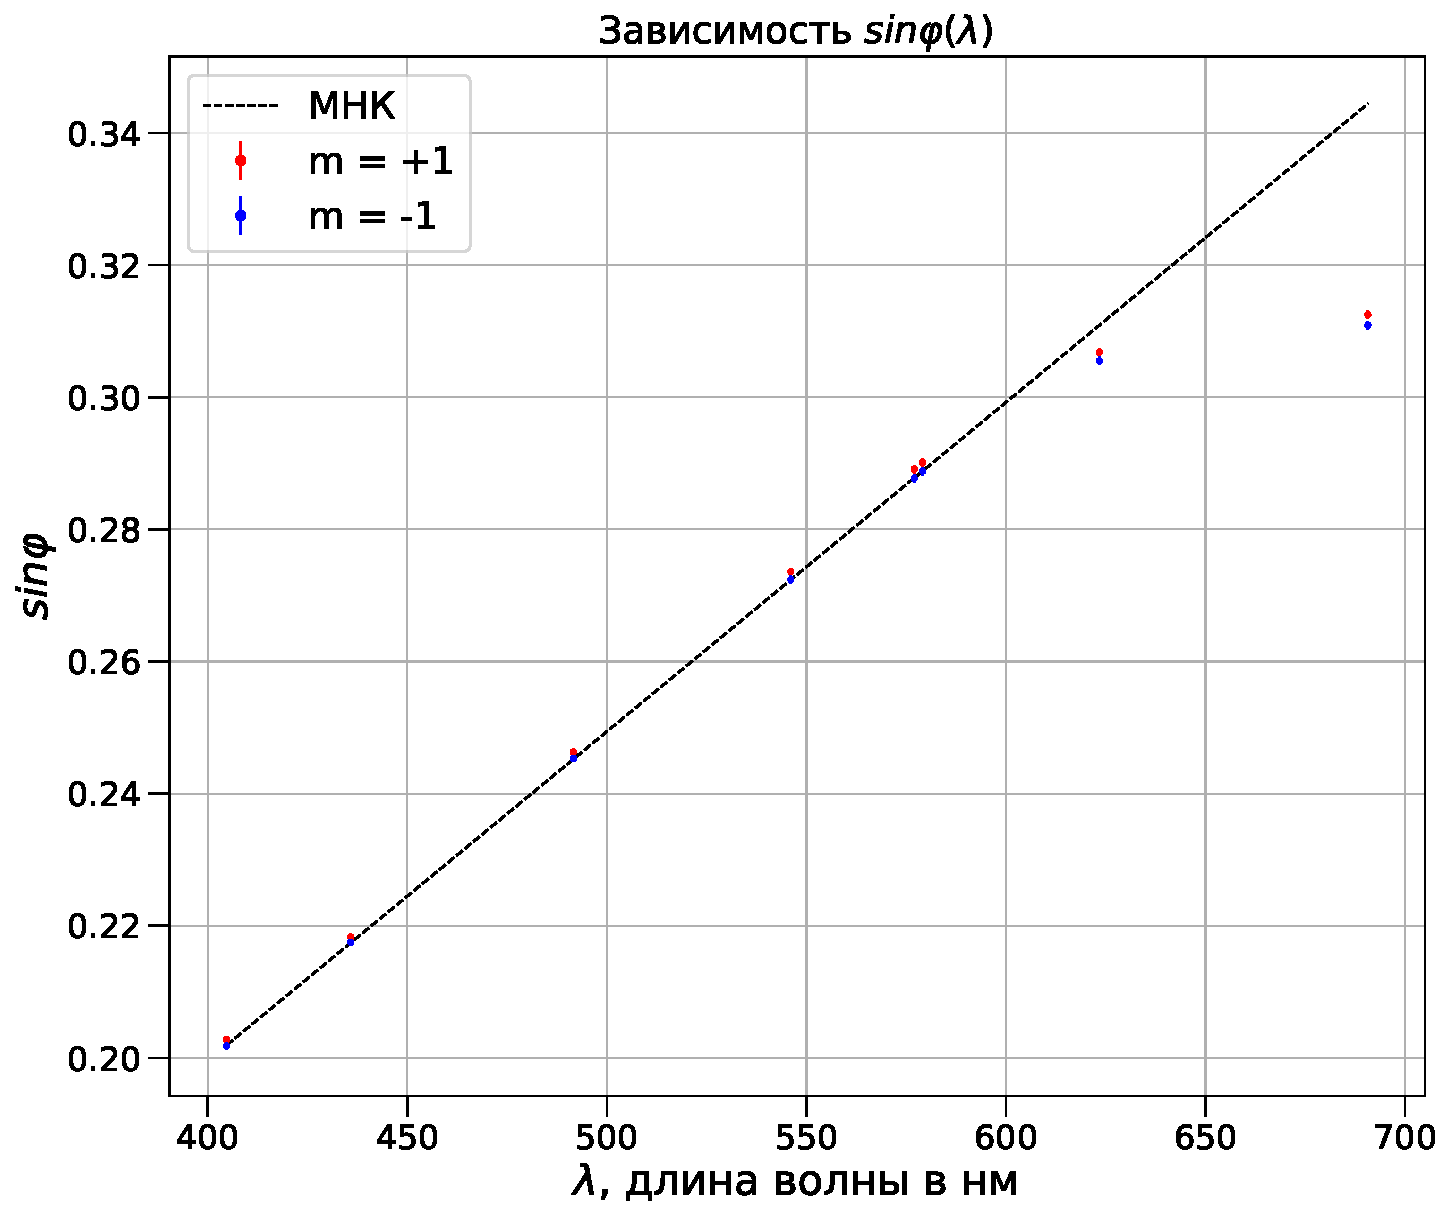
\includegraphics[scale=0.65]{4.4.1/sin.pdf}
    \caption{График зависимости $\sin \varphi$ от длины волны для первых максимумов}
    \label{angle}
\end{figure}

Далее, посмотрим зависимость $D$ от $m$ и сравним результат с формулой 2. Результат наглядно представлен на графике \ref{D}.

\begin{figure}[H]
    \centering
    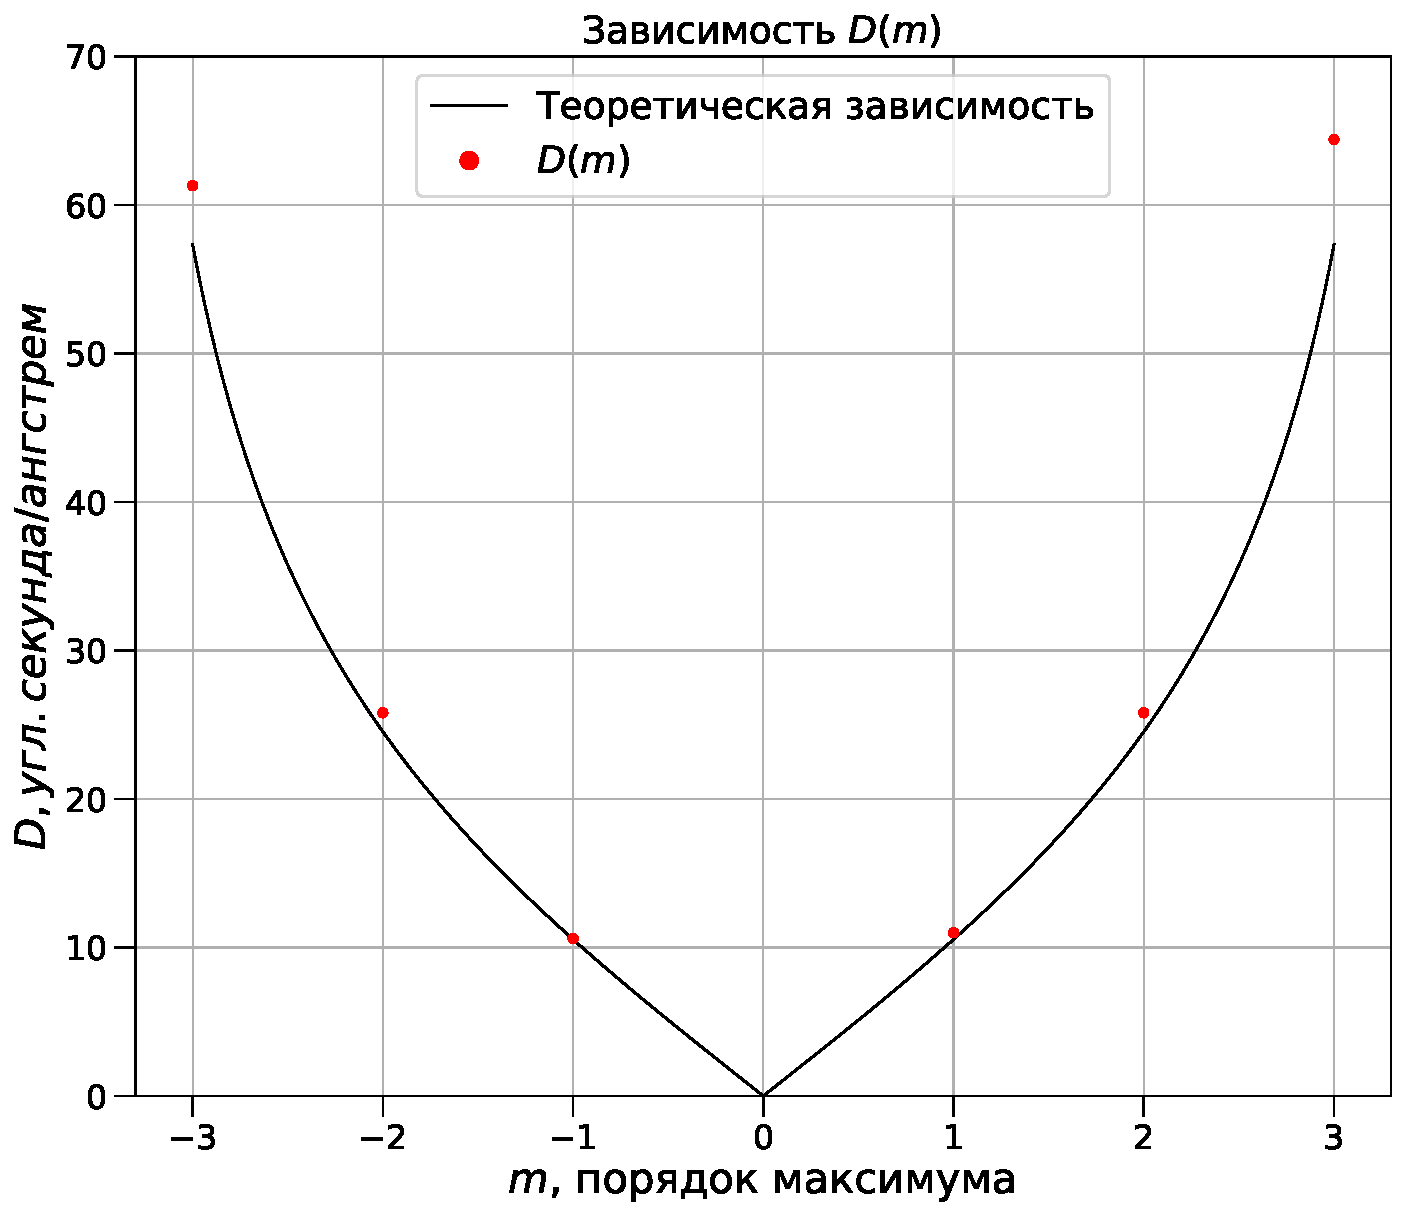
\includegraphics[scale=0.65]{4.4.1/D.pdf}
    \caption{\centering Зависимость угловой дисперсии от порядка. Черная прямая - это теоретическая зависимость, построенная по параметру $d$, ранее определенному. Легко видеть, что теория очень хорошо описывает эксперимент}
    \label{D}
\end{figure}

Определим также разрешающую способность по формуле $\displaystyle R = \frac{\varphi}{\delta \varphi} \approx 670$, используя измеренную ширину первого порядка жёлтой линии $\delta \varphi = 90^{ \prime \prime }$, то есть число рабочих штрихов решётки $N \approx 670$ и размер освещённой части $l = Nd \approx 1,3$ мм.

\section{Вывод}

Таким образом, мы исследовали спектральные линии ртути, определили шаг решётки, её угловую дисперсию, а также её разрешающую способность. Полученные результаты близки к теоретическим вычислениям.

\end{document}
